\section{问题3：全向源的在线定位与清除}

\subsection{目标、信息集与完备性}

问题3中全部干扰源为全向，总数 $N\in\{10,\ldots,16\}$ 在线未知。机器狗从原点出发，测向机初始频道为 $1$。字典序目标是先保证 $K=N$，再尽量缩短虚拟时间 $T$。正式测试永不返回 $N$，因而不能把“已经清除 $10$ 个”写成结束条件，也不能在表1里用 $K$ 冒充清除比例。二十个频道并不都有源，单点二十频道无信号更不能代替频道判空。

单点测向无法同时看见所有源。传感器网络文献把检测、分类与跟踪分成层次\upcite{li_2002_tracking}；本题只有单机、单频道，层次被压成“发现覆盖 $\to$ 局部交会 $\to$ 光学清除 $\to$ 频道判空”。覆盖路径规划强调：保证扫过工作区域的点集或轨迹，与之后的时间优化是两件事\upcite{galceran_2013_cpp}。定向越野把收益顶点放进时间预算\upcite{vansteenwegen_2011_op}，但本题收益是未知频道上的首次 $\mathtt{direction}$ 或 $\mathtt{near}$，预算是虚拟时间，且漏清不可用超时换取。因此本节先给出发现点集，再给出局部定位与光学兜底，最后才用非正式演练比较策略，正式成绩表保持空缺。

\subsection{七点发现覆盖}

取
\begin{equation}
P_3=\bigl\{(0,0)\bigr\}\cup\bigl\{1200(\cos(j\pi/3),\sin(j\pi/3)):j=0,\ldots,5\bigr\}.
\end{equation}
对任意 $g\in\Omega$，$\|g\|\le 1800$。原点到 $g$ 可能超过 $1000\,\mathrm{m}$，但六个顶点把圆域分成六个 $60^\circ$ 扇。$g$ 到最近 $P_3$ 点的距离不超过 $1200\,\mathrm{m}$ 量级的网格半径；更紧的是：半径 $1800$ 的圆被半径 $1200$ 的正六边形顶点加中心覆盖时，任意点到该七点的距离不超过 $1200\,\mathrm{m}$（中心到顶点 $1200$，顶点之间 $1200$，圆边界落在相邻顶点的 Voronoi 内时距离更短）。$1200$ 落在 $[1000,1500]$ 内，对 $r_i\ge 1200$ 的源，最近点一定可测；对 $r_i\in[1000,1200)$ 的源，原点附近与边界附近仍可能需要后续局部测向。因此 $P_3$ 是发现层的充分网格，而不是对一切 $r_i$ 的单点可测证书。实现上巡回这七点，每点扫描尚未清除且尚未判空的频道。同站先批量扫描，避免“测到一个方向就离开、下一频道再折返”。

七点之间的边长为 $1200\,\mathrm{m}$，按 $5\,\mathrm{m/s}$ 行走约 $240\,\mathrm{s}$。
若每站对尚未判空的频道各测一次，检测时间随未决频道数线性增加，切换 $1\,\mathrm{s}$ 只在频道改变时支付。
巡回顺序取原点出发、沿六边形边界再回到原点附近处理残留，避免为了理论最短 Hamilton 回路而在线搜索。
对 $r_i\ge 1200$ 的源，最近 $P_3$ 点落入接收球；对更短的接收半径，第一次 $\mathtt{no\_signal}$ 只说明该站不可测，必须把后续局部测向与 SAFE 走廊当作完备性的第二层，而不是宣称七点已经单点可测一切源。
这一点与问题4的格点证书不同：后者对最小接收半径 $1000\,\mathrm{m}$ 给出严格存在性，前者对全向源给出实用发现网格。
原点本身对圆域中心附近的源几乎总是可测，六个顶点则负责贴边源；二者缺一，边界附近就会留下接收半径刚过 $1000\,\mathrm{m}$ 却距七点都远的死角。
同站批量扫描的代价是检测时间随未决频道上升，收益是避免旧版那种拿到一个方向就离开、下一频道再折返的往返。

判空规则与问题4不同。问题3在已经确认某频道仍有未清除全向源时，可把 $\mathtt{no\_signal}$ 读成 $d>r_i$；对从未出现过正观测的频道，必须在全部发现点上无信号才倾向判空，并且不能用“已清 $10$ 个”代替。主线策略把发现巡回走完，再用局部后验与光学走廊处理残留。$N=16$ 时十六个不同频道一旦都出现正观测，其余四频道可由计数判空，这是计数证书而不是几何证书；当前实现仍走完发现点，以免把计数与几何混成提前停机。

\begin{figure}[H]
\centering
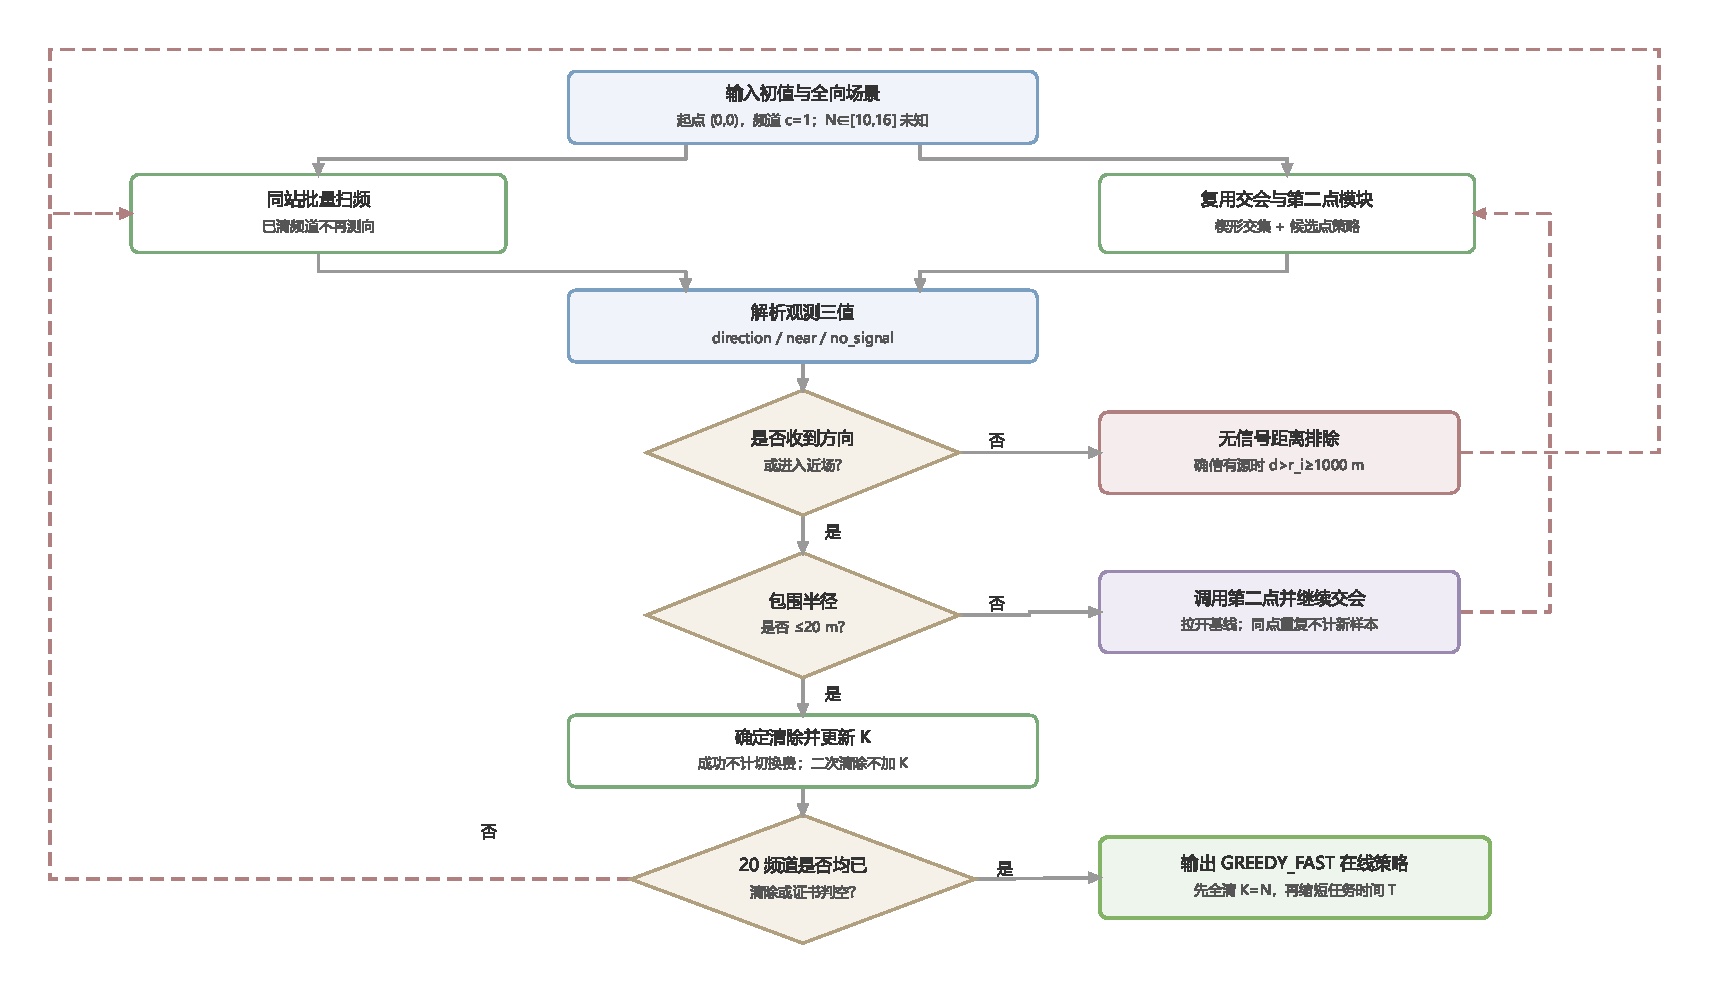
\includegraphics[width=0.82\textwidth,height=0.52\textheight,keepaspectratio]{../figures/fig_flow_q3.pdf}
\caption{问题3在线清除流程}
\label{fig:flow_q3}
\end{figure}

在线闭环的主干是走完 $P_3$ 巡回并在每站扫描未决频道。
已发现频道进入第二测点与试清。
后验足够小时改用光学网格或 SAFE 走廊兜底。
全部频道为已清除或证书判空时才退出。
图中右侧回路把巡回未完成与局部未清完分开，避免启发式预算把机器狗永久停在半途。
源预算参数 $\mathrm{SourceBudgetS}=0$，即不以启发式耗尽作为停机条件。
GREEDY\_ABORT 曾把预算超限写成放弃该源，演练中全清率降至 $1/10$，正是这条回路被切断的后果。

\subsection{局部定位与 GREEDY\_FAST}

发现某频道的第一次 $\mathtt{direction}$ 后，调用问题2的几何。
沿示向度前进约 $500\,\mathrm{m}$ 并横向偏移 $150\,\mathrm{m}$ 取第二测点。
若当前位姿已经满足沿向 $\ge 200\,\mathrm{m}$ 且横向 $\ge 80\,\mathrm{m}$，则就地作为第二点，以免离开巡回。
两次示向度的楔形交给出后验多边形，包围半径不超过 $20\,\mathrm{m}$ 时在圆心清除。
半径略大于 $20\,\mathrm{m}$ 时允许一到两次中心试清，失败不禁止后续确定清除。
沿向 $500\,\mathrm{m}$、横向 $150\,\mathrm{m}$ 不是问题2演示点 $q^\ast$ 的现场拷贝，而是巡回途中可计算的固定偏移，避免为理论最优点破坏七点顺序。

$\mathtt{near}$ 在原地立即光学清除。已清除频道不再扫描。同点同频道重复测量仍支付时间，但不提供新的独立误差样本，策略禁止把重复测量当成加密。累计观测时把新的楔形裁进已有凸多边形，数值半宽取 $1.005^\circ$ 以吸收两位小数量化，物理误差仍为 $1^\circ$。

回退基线 GREEDY 在发现后立即插入较重的局部射线与试清，巡回中 SAFE 走廊触发较多。主线 GREEDY\_FAST 把发现期的投机试清关掉，把尾部交给显式有界求解器；源预算参数 $\mathrm{SourceBudgetS}=0$。GREEDY\_ABORT 曾把预算超限写成放弃该源，演练中全清率降至 $1/10$，不作正式候选。预算模式 $\mathrm{SourceBudgetS}=300$ 也不作为主线。GREEDY 保留为回退基线，代码快照在稳定目录中，正式入口默认 GREEDY\_FAST。

当后验多边形仍大于光学半径时，启用 SAFE 走廊：在示向度坐标系下取纵向 $A=10,30,\ldots,1490\,\mathrm{m}$，横向 $B\in\{-20,0,20\}$，共 $75\times 3=225$ 个点，按“$B=-20$ 前进、$B=0$ 折返、$B=+20$ 再前进”的蛇形顺序走。相邻点间距 $20\,\mathrm{m}$，走廊半宽 $20\,\mathrm{m}$，用以覆盖楔形中可能的源位。若后验已经是小凸集，则改用边长 $28\,\mathrm{m}$ 的主轴方格：半对角线 $14\sqrt{2}<20\,\mathrm{m}$，方格与多边形的非空交集被一个半径不超过 $20\,\mathrm{m}$ 的圆覆盖，从而光学点覆盖的是连续区域而不是采样点。走廊与方格都是有界兜底，走完仍无成功则报告模型与数据不一致，不把该频道改写成证书缺席。

SAFE 走廊的纵向取到 $1490\,\mathrm{m}$，是因为接收半径上界为 $1500\,\mathrm{m}$，再往远处走已经离开可能的射频覆盖；横向 $\pm 20\,\mathrm{m}$ 与光学半径相同，使相邻蛇形列能够把楔形中可能的源位盖住。
走廊不是最短路：它是有界搜索，最坏情况下要走完 $225$ 点。
纵向步长 $20\,\mathrm{m}$ 与横向三列合在一起，使相邻点间距不超过光学直径，从而走廊扫过的是连续条带而不是离散抽样。
GREEDY\_FAST 把发现期投机试清关掉，正是为了少触发这条走廊；演练里 SAFE 均值从 $1.20$ 降到 $0.20$，对应的是更少进入尾部搜索，而不是把 $225$ 点删掉。
光学方格只在后验已经是小凸集时启用，避免在尚未收缩的大楔形上铺满 $28\,\mathrm{m}$ 格子。
两种兜底都覆盖连续区域：走廊用 $20\,\mathrm{m}$ 间距加 $20\,\mathrm{m}$ 半宽，方格用半对角线小于 $20\,\mathrm{m}$。
点抽样式试清不在主线里，因为它不能证明区域搜完。
启发式预算不得升级为永久放弃：ABORT 把预算超限写成停机后全清率降至 $1/10$，正是走廊与方格被切断的后果。
源预算参数 $\mathrm{SourceBudgetS}=0$ 表示主线不以启发式耗尽作为停机条件；预算模式 $300$ 同样不作为主线。

\subsection{非正式演练对照}

同晚十局演练（非配对、非正式）把三条策略放在同一入口下对照，结果见表~\ref{tab:q3_practice}。主线相对 GREEDY 的平均 $T/K$ 下降来自更少的走廊插入，而不是放弃完备性。ABORT 的全清失败表明：预算一旦写成永久停机，覆盖证书就被破坏。这些数字只用于策略筛选，禁止填入表1。

\begin{table}[H]
\centering
\caption{问题3非正式演练策略对照}
\label{tab:q3_practice}
\begin{tabular}{lcccc}
\hline
策略 & 全清 & 平均 $T/K$ & 区间 & SAFE均值 \\
\hline
GREEDY & $10/10$ & $390$ & $334$--$455$ & $1.20$ \\
GREEDY\_FAST & $10/10$ & $341$ & $244$--$450$ & $0.20$ \\
GREEDY\_ABORT & $1/10$ & $382$ & $295$--$482$ & $0$ \\
\hline
\end{tabular}

\vspace{0.4em}
{\small 同晚十局，场景随机非配对，非正式。禁止写入表~\ref{tab:q3_formal}。}
\end{table}

GREEDY\_FAST 另十局轨迹上 $T/K$ 落在 $[243.74,449.50]$，均值 $340.98\,\mathrm{s}$，与发表表中的 $341\,\mathrm{s}$ 一致（发表表取整）。
十局均 $K=N$ 且证书完成。
场景随机，不能解释成置信区间，也不能单独支撑相对 GREEDY 改进百分之多少的因果断言。
墙钟侧的 UIA 启动偶发误超时与虚拟时间不是同一问题，却可能吃掉正式测试额度，正式入口因此与演练入口分开。
三条策略放在同一晚、同一入口下，是为了控制操作差异，不是为了制造配对种子。

\begin{figure}[H]
\centering
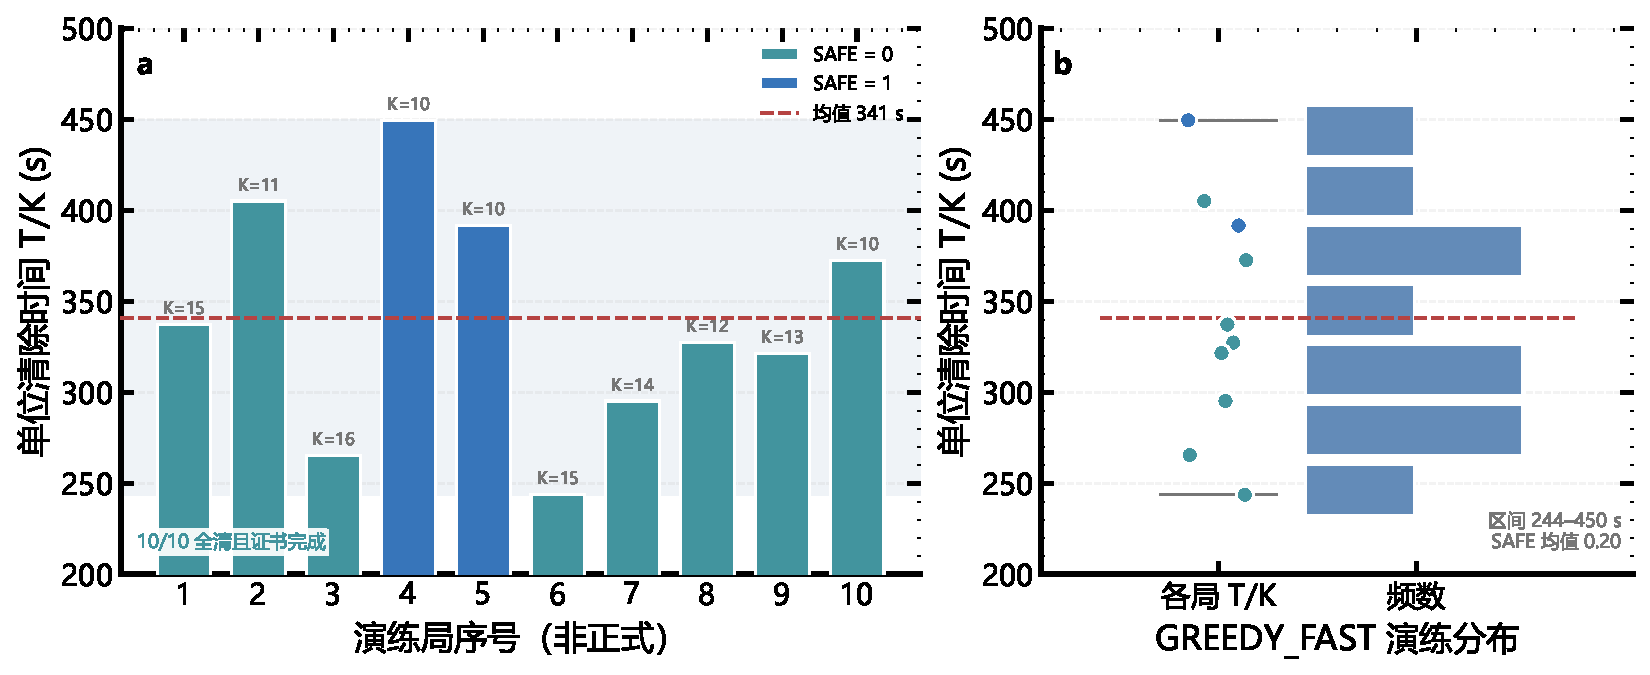
\includegraphics[width=0.95\textwidth,height=0.9\textheight,keepaspectratio]{../figures/fig_q3_practice_tk.pdf}
\caption{GREEDY\_FAST演练$T/K$}
\label{fig:q3_practice_tk}
\end{figure}

左面板按局给出单位清除时间，右面板给出其分布。
离散点全部落在大约 $240$ 至 $450\,\mathrm{s}$ 之间，没有出现 $K=0$ 的未定义点，也没有出现远高于 GREEDY 区间上沿 $455\,\mathrm{s}$ 的异常局。
与发表表中取整后的 $341\,\mathrm{s}$ 对照时，应以该分布的均值 $340.98\,\mathrm{s}$ 为同一批轨迹的未取整记录。
分布宽度约 $200\,\mathrm{s}$ 来自源的几何散布与发现顺序，而不是随机数种子可重复的置信区间。
口径是非正式演练，场景非配对，不得写入正式测试表。
区间下沿 $244\,\mathrm{s}$ 低于 GREEDY 的 $334\,\mathrm{s}$，上沿 $450\,\mathrm{s}$ 与 GREEDY 的 $455\,\mathrm{s}$ 接近，说明加速主要发生在走廊较少的局，而不是把所有局都削去同一常数。

\begin{figure}[H]
\centering
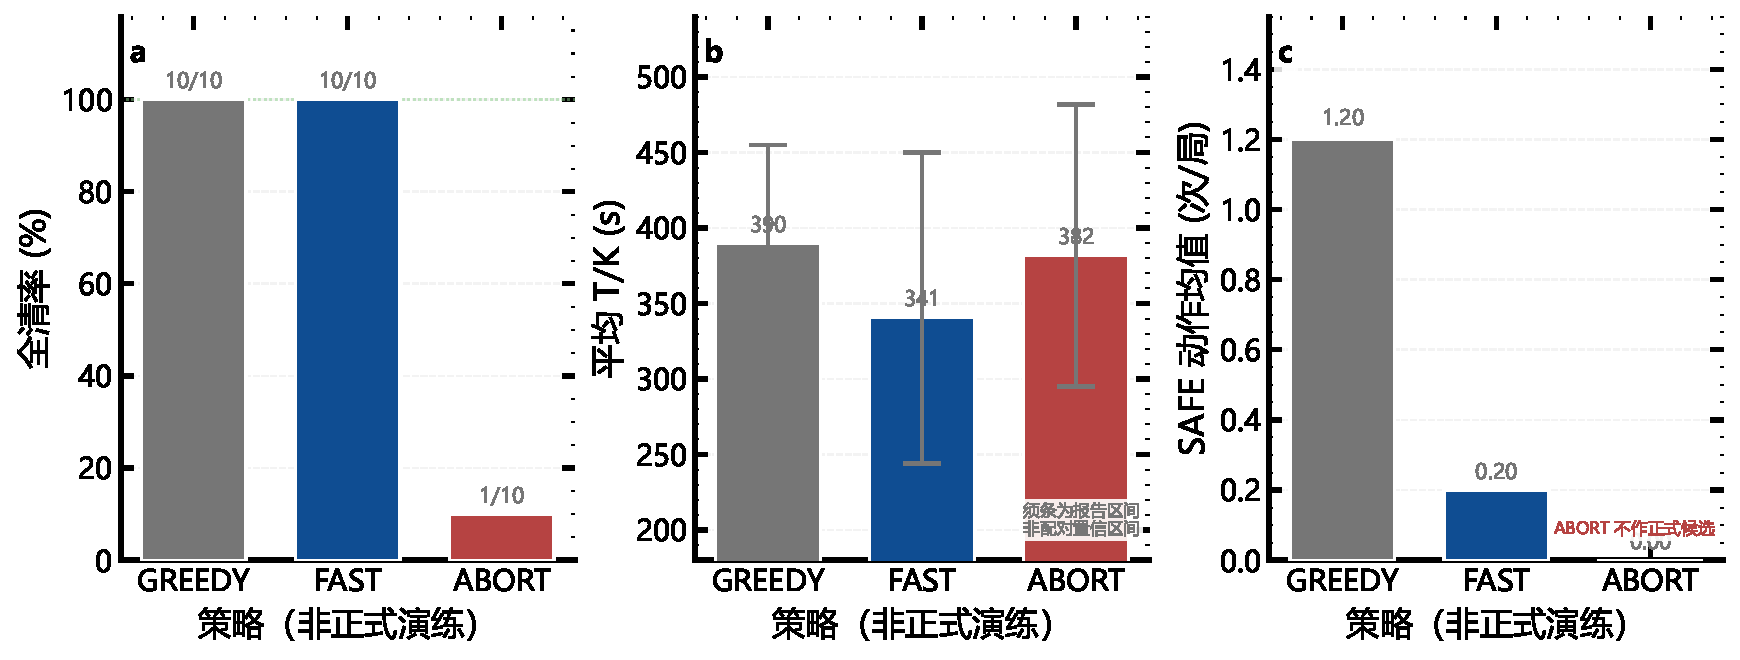
\includegraphics[width=0.95\textwidth,height=0.9\textheight,keepaspectratio]{../figures/fig_q3_strategy.pdf}
\caption{问题3策略对照}
\label{fig:q3_strategy}
\end{figure}

全清率、平均 $T/K$ 与 SAFE 均值三条对照把 ABORT 排除出正式候选。
它在全清率上不可接受，平均时间 $382\,\mathrm{s}$ 接近 GREEDY 并不能补偿漏清。
GREEDY 保留为回退基线，因为它仍然 $10/10$ 全清，只是走廊插入更多、平均 $T/K$ 为 $390\,\mathrm{s}$，区间 $334$--$455$，SAFE 均值 $1.20$。
主线 GREEDY\_FAST 把 SAFE 均值从 $1.20$ 降到 $0.20$，同时保持全清，说明时间收益来自更少的走廊，而不是把启发式预算升级为停机。
对照局间场景独立，不是配对种子，不能把 $341$ 对 $390$ 的差值写成竞赛期望改进。
预算模式 $\mathrm{SourceBudgetS}=300$ 同样不作为主线：它把启发式耗尽写成停机，与 ABORT 同类。

\subsection{正式测试结果}

问题3正式测试尚未执行，额度为独立三次。表~\ref{tab:q3_formal} 按题面格式列出，单元格保持空缺。程序运行时间指 $\mathtt{/enter}$ 至结束的墙钟，与虚拟 $T$ 不是同一列。中止测试仍占用一次额度。截止时间之后不能启动新的正式测试；本文不把演练日志改名充当正式日志。主线策略没有在官方正式模块上验证，截止之后不能补做。

\begin{table}[H]
\centering
\caption{问题3正式测试结果}
\label{tab:q3_formal}
\begin{tabular}{cccc}
\hline
测试案例编码 & 清除干扰源个数 & 平均定位清除时间 & 程序运行时间 \\
\hline
测试1案例编码 & --- & --- & --- \\
测试2案例编码 & --- & --- & --- \\
测试3案例编码 & --- & --- & --- \\
\hline
\end{tabular}

\vspace{0.4em}
{\small 正式测试未执行。表中“---”表示缺失，不是零。禁止用演练 $T/K$ 或离线几何模型填入。}
\end{table}

空缺不是把非正式 $341\,\mathrm{s}$ 四舍五入后的占位。
第四列若将来有数，也只报告墙钟，不得把虚拟 $T$ 抄过去。
三次额度用尽或截止时间 $2026$ 年 $9$ 月 $13$ 日 $17$:$30$ 之后，本文不再补行。
主线 GREEDY\_FAST 的正式表现因此保持未知，评价章把这一点列为主要局限。
问题3额度与问题4独立，互不占用；中止一次即少一次正式机会。
入口脚本与正式模块分开：演练入口拒绝正式模式，避免一次误点占用额度。
墙钟侧的 UIA 启动偶发误超时与虚拟账本无关，却可能把一次正式机会耗掉，因此正式启动必须与演练核对入口分离。
字典序下全清优先于平均时间：ABORT 的 $1/10$ 已经足够否决该候选，不必再讨论 $382\,\mathrm{s}$ 是否碰巧接近 GREEDY。
预算模式 $\mathrm{SourceBudgetS}=300$ 与 ABORT 同类，同样不进入正式入口。
GREEDY 快照保留在稳定目录，只作回退基线，不与主线并行提交。
